\documentclass{article}
\usepackage{../fasy-hw}

%% UPDATE these variables:
\renewcommand{\hwnum}{5}
\title{Advanced Algorithms, Homework \hwnum}
\author{Ben Miller}
\collab{\todo{list your collaborators here}}
\date{due: Monday, 8 November 2021}

\begin{document}

\maketitle

This homework assignment should be
submitted as a single PDF file both to D2L and to Gradescope.

General homework expectations:
\begin{itemize}
    \item Homework should be typeset using LaTex.
    \item Answers should be in complete sentences and proofread.
    \item You will not plagiarize, nor will you share your written solutions
        with classmates.
    \item List collaborators at the start of each question using the
        \texttt{collab} command.
    \item Put your answers where the \texttt{todo} command currently is (and
        remove the \texttt{todo}, but not the word \texttt{Answer}).
    \item If you are asked to come up with an algorithm, you are
        expected to give an algorithm that beats the brute force (and, if possible, of
        optimal time complexity). With your algorithm, please provide the following:
        \begin{itemize}
            \item \emph{What}: A prose explanation of the problem and the algorithm,
                including a description of the input/output.
            \item \emph{How}: Describe how the algorithm works, including giving
                psuedocode for it.  Be sure to reference the pseudocode
                from within the prose explanation.
            \item \emph{How Fast}: Runtime, along with justification.  (Or, in the
                extreme, a proof of termination).
            \item \emph{Why}: Statement of the loop invariant for each loop, or
                recursion invariant for each recursive function.
        \end{itemize}
\end{itemize}

\collab{\todo{}}
\nextprob{The Skyline Problem}

You are in Camden, NJ waiting for the ferry across the river to
get into Philadelphia, and are looking at the skyline.  You take a photo, and notice that each building
has the silhouette of a rectangle.  Suppose you  represent each building $b$ as a
triple $(x_b^{(1)},x_b^{(2)},y_b)$, where the building can be seen from $x_b^{(1)}$ to $x_b^{(2)}$
horizontally and has a height of $y_b$.  Let $\mathtt{rect(b)}$ be the set of
points inside this rectangle (including the boundary).  Let $\mathtt{buildings}$
be a set of $n$ such triples representing buildings. Design an algorithm that takes $\mathtt{buildings}$ as input, and
returns the skyline, where the skyline is a sequence of~$(x,y)$ coordinates
defining $\cup_{b \in \mathtt{buildings}} \mathtt{rect}(b)$.  The output should
start with $(\min_b{x_b^{(1)}},0)$ and end with $(\max_b{x_b^{(1)}},0)$.

\paragraph{Answer}

For this problem, we'll first sort the buildings by the left boundary. Then, we'll
iterate through each building and perform the following steps:

1. Add the ($x_b^{(1)}$,$y_b$) coordinate to the skyline if the current building is taller than the current height and advance
x_{skyline} to.\\
2. Add the ($x_b^{(2)}$,$y_b$) coordinate to a priority queue based on the height.


\todo{}

\collab{}
\nextprob{Longest Increasing Subsequence}

Next, we consider the problem of finding the longest increasing subsequence.

\begin{enumerate}
    \item
        Walk through one of the exponential time algorithms to compute the
        Longest Increasing Subsequence (LIS) for the input: $\left[ 1, 7, 6, 11,
        3, 11 \right]$.  You can use either the algorithm presented in 2.6 or
        the algorithm presented in 2.7.

        \paragraph{Answer}
        2.7
        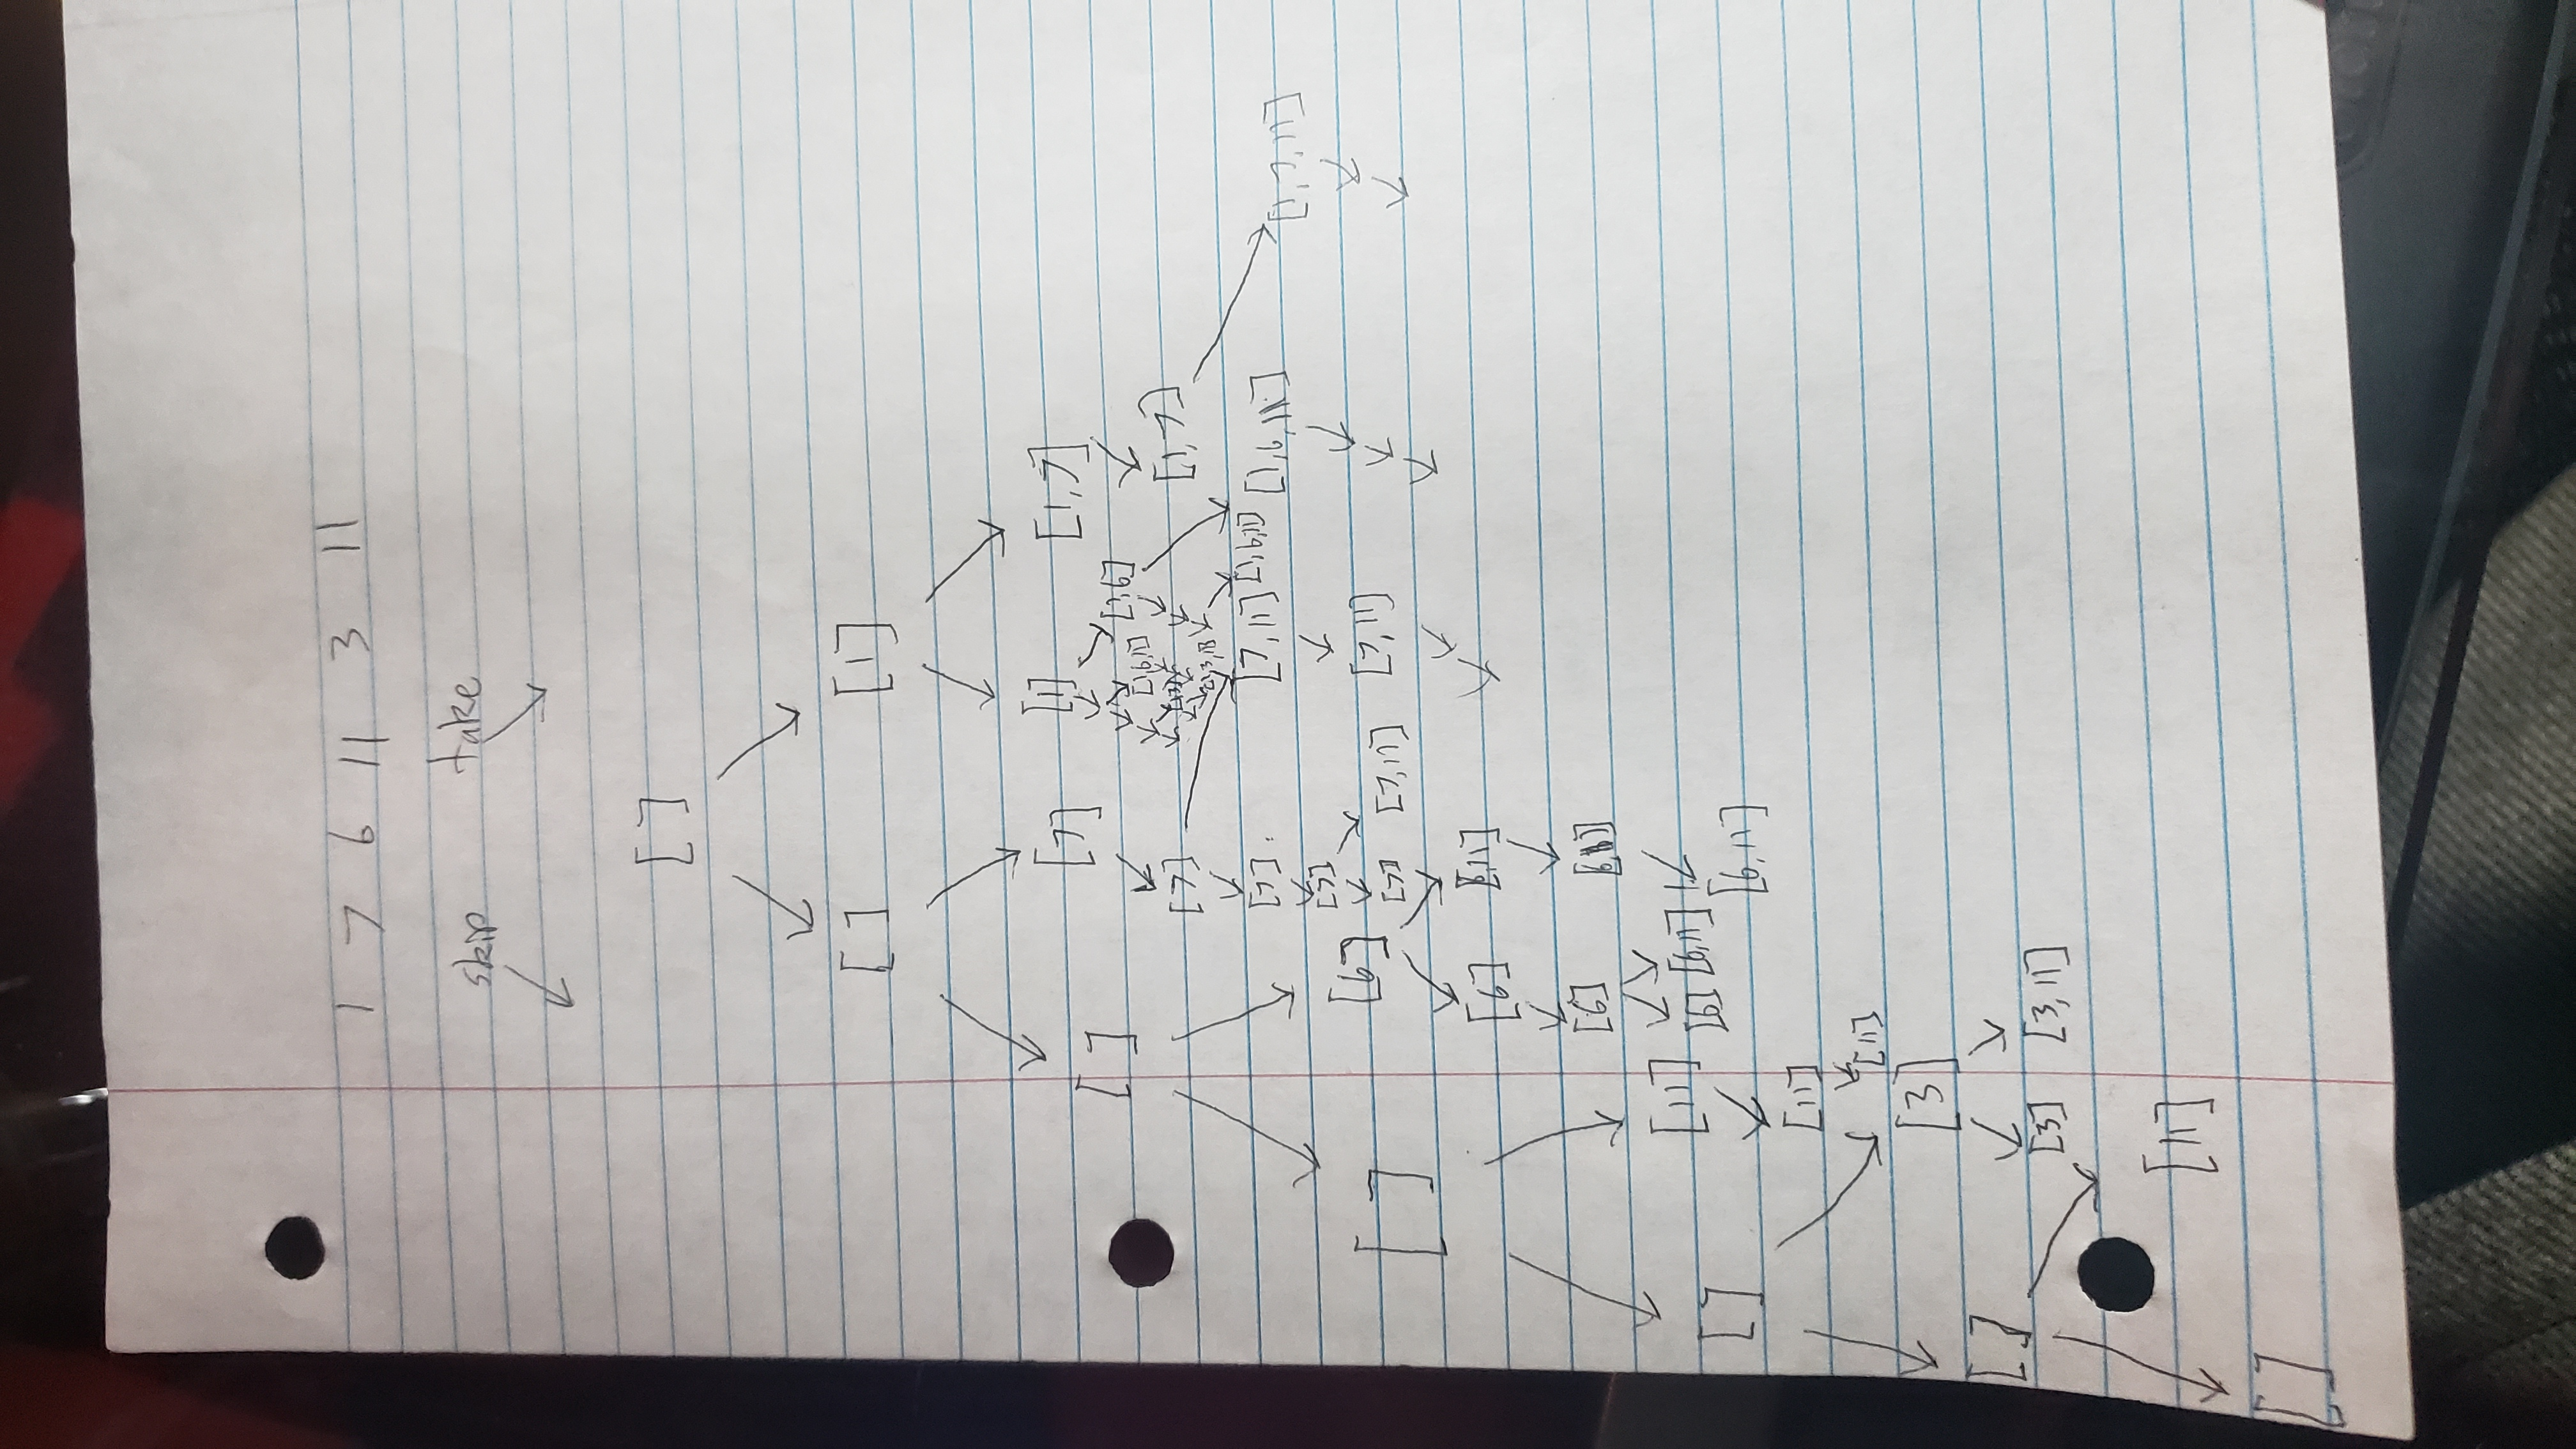
\includegraphics[width=400,height=400,keepaspectratio,angle=-90]{BruteForceLIS.jpg}

    \item
        Walk through the algorithm (on the same input) using the Dynamic Programming algorithm
        present in Section 3.6.\\
        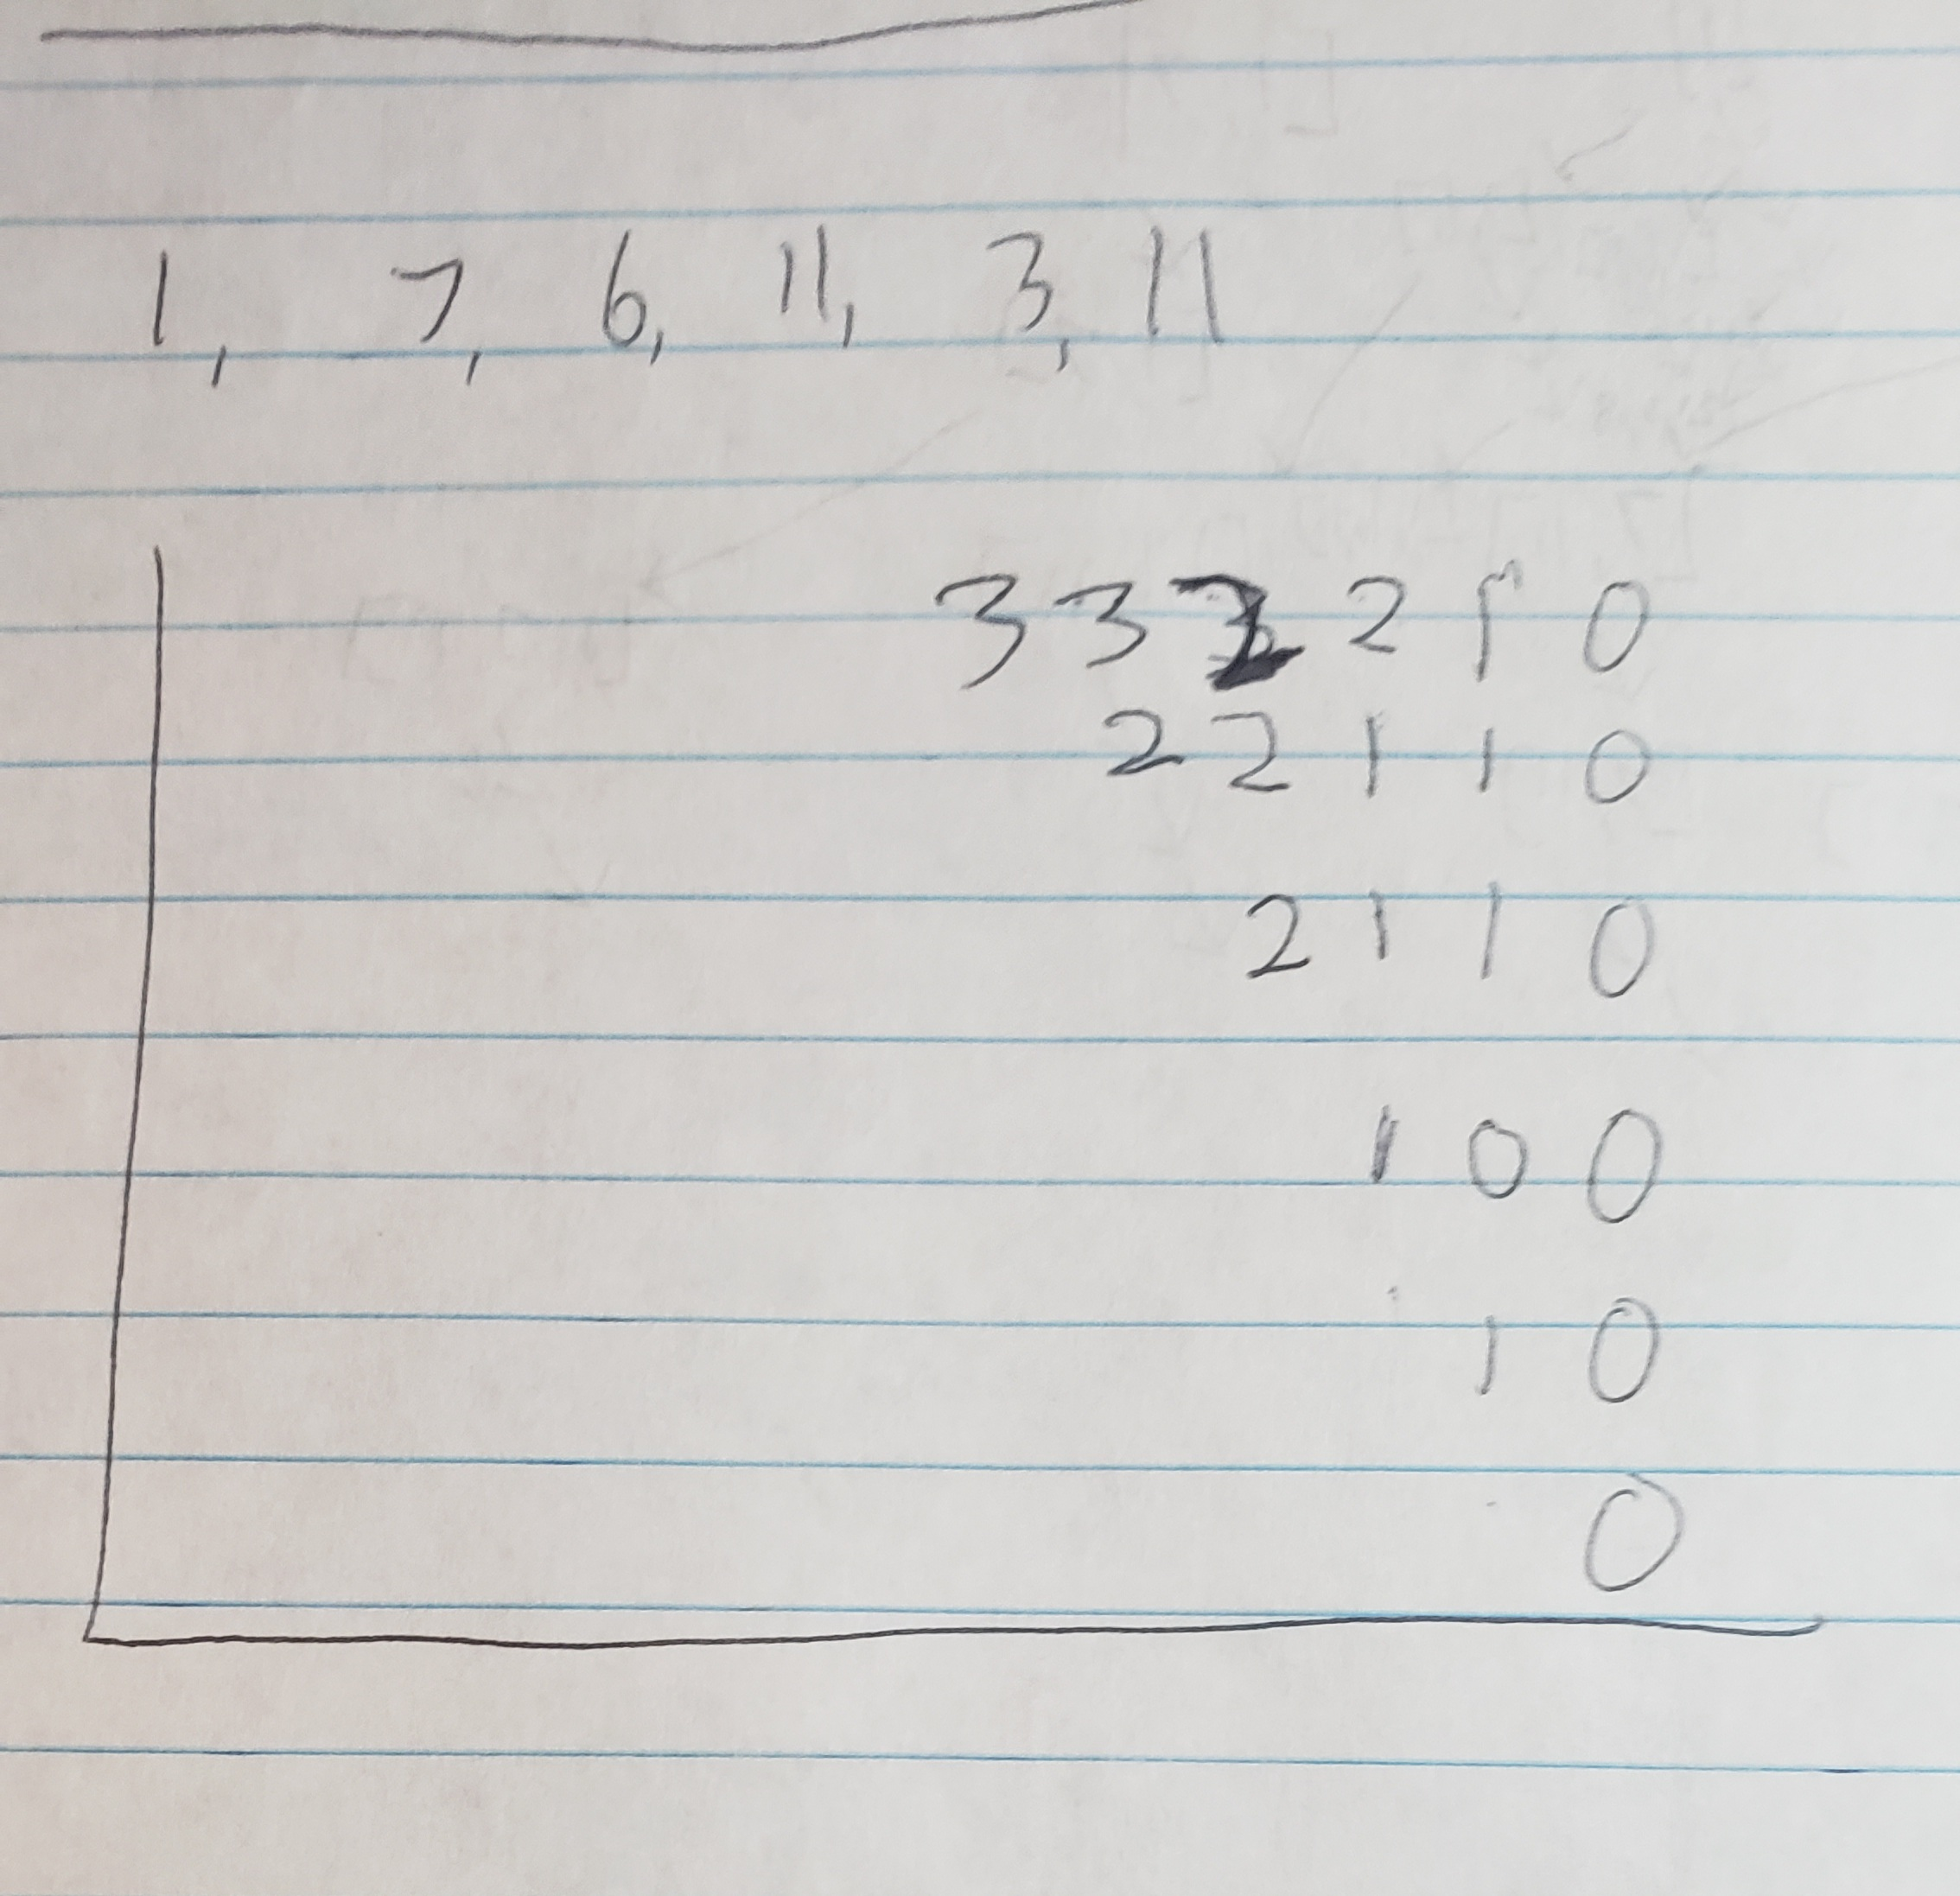
\includegraphics[width=400,height=400,keepaspectratio]{DynamicLIS.jpg}

\end{enumerate}

\collab{\todo{}}
\nextprob{Decrementing Function}

Consider the algorithm \textsc{StrongComponents} given on in Figure 6.15 of the
textbook. Notationally, use $G=(V,E)$ for the graph and let $n=|V|$ and $m=|E|$.
In the for loop, there are at most $n$ vertices that will be
considered. So, that loop will terminate in $O(m)$ iterations.
Use a decrementing function to prove that the while loop terminates.

\paragraph{Answer}

$StrongComponents: D \rightarrow \mathbb{N}$

If a vertex has no outgoing edges it is a sink. In each loop of the while loop,
a vertex from a sink component is found and every vertex reachable in that sink
component is removed. For each loop, $n = n - k$ with $k >= 1$ and $m= m -j$ with $j >= 1$

In removing a sink component, a new sink component is always created until there
are no more vertices.

The statespace of StrongComponents decreases in each iteration of the while loop.
Therefore it will terminate.

\collab{}
\nextprob{Kruskal}

Walk through Kruskal's algorithm, using the graph in Figure 7.7 (left) of the
textbook.  Label the center vertex $a$, the other red vertex $b$, and the
remainder $c$ through $g$ in counter-clockwise order.  You should use the
union-find data structure, with both ``heuristics.''

\paragraph{Answer}

a, b, c, d, e, f, g

a, a, c, d, e, f, g
2, 1, 1, 1, 1, 1, 1

a, a, c, a, e, f, g
2, 1, 1, 1, 1, 1, 1

a, a, c, a, e, g, g
2, 1, 1, 1, 1, 1, 2

a, a, b, a, e, g, g
3, 2, 1, 1, 1, 1, 2

a, a, b, a, e, g, a
3, 2, 1, 1, 1, 1, 2

a, a, b, a, d, g, a
3, 2, 1, 2, 1, 1, 2

\todo{}

\collab{}
\nextprob{Maximum and Minimum Edges in Cycles}

Chapter 7, Question 1

1. Let G = (V, E) be an arbitrary connected graph with weighted edges.

(a) Prove that for any cycle in G, the minimum spanning tree of G excludes
the maximum-weight edge in that cycle.

(b) Prove or disprove: The minimum spanning tree of G includes the
minimum-weight edge in every cycle in G.

\begin{enumerate}[(a)]

    \item Excluding Maximum Weight Edges.

        \paragraph{Answer}

        We will prove this by contradiction

        \begin{proof}

            Assume that the maximum-weight edge in a cycle is in the minimum spanning
            tree.

            Let G' be a subgraph of G where every vertex $v_{i}$ and edge $e_{i}$ in G'
            is in a cycle in G. let W be the total weight of G'.

            Because G' is a cycle, every $v_{i}$ can be reached by two edges.
            Because we have included the maximum weight edge, we have excluded
            another edge. The total weight of G' with the can be written $W = W -
            weight(e_{max}) + weight(e_{max})$, while if we were to use a different
            edge other than $e_{max}$, the total weight of G' would be written as
            $W = W - weight(e_{max}) + weight(e_{i})$. Because $weight(e_{max}) > weight(e_{i})$, W would be smaller with $e_{i}$ than with $e_{max}$.

            Therefore, the minimum spanning tree excludes the maximum-weight
            edge in a cycle.

        \end{proof}


    \item Including Minimum Weight Edges.

        \paragraph{Answer}

        We will disprove this statement by contradiction.

        \begin{proof}
            Let G' be a cycle in G.

            For this example, we will set all weights of G' to 4 and one edge
            weight to 3 that we'll call $e_{3}$. Let one vertex connect to the vertices on either side
            of $e_{3}$ with weights of 1 each. This new cycle will be called G".

            The minimum spanning tree will contain the two edges with weights of 1
            and will skip $e_{3}$, which is the minimum weight edge in G'.

            Therefore, not every minimum-weight edge in every cycle in G is in
            the minimum spanning tree of G.
        \end{proof}

\end{enumerate}


\collab{}
\nextprob{Maximum Weight Spanning Tree}

Chapter 7, Question 4, Part(a).

Describe and analyze an algorithm to compute the maximum-weight
spanning tree of a given edge-weighted graph

\paragraph{Answer}

This problem is akin to running a regular minimum spanning tree algorithm on
a Graph with the inverse of all the edges. We just consider a safe edge to be
the largest edge going away from each vertex. So, we'll do the Boruvka method;
we'll add all the safe edges and recurse.

Because this algorithm is the exact same as Boruvka's but with the safe edges inverted,
the runtime and proof of the algorithm is the exact same. For a detailed discussion
on analysis and proof of this algorithm, see Jeff Erickson's "Algorithms" at page 262.

The running time is $O(E log V)$

\end{document}
